\documentclass[12pt]{article}
\usepackage[a4paper, left=2cm, right=2cm, top=3cm, bottom=3cm]{geometry}
\usepackage{graphicx}
\usepackage{pdflscape}
\usepackage{float}
\usepackage{listings}

\graphicspath{{img}}
\pagenumbering{gobble}

\title{\vspace{4cm}\Huge{Profiling the calculator} \\ \vspace{1cm} \LARGE{Results report}\vfill}
\author{Patrik Skaloš, xskalo01 \vspace{5cm}}
\date{}

\begin{document}

  \begin{landscape}
    \begin{titlepage}
      \maketitle
    \end{titlepage}
  \end{landscape}


    \begin{figure}
      \begin{center}
        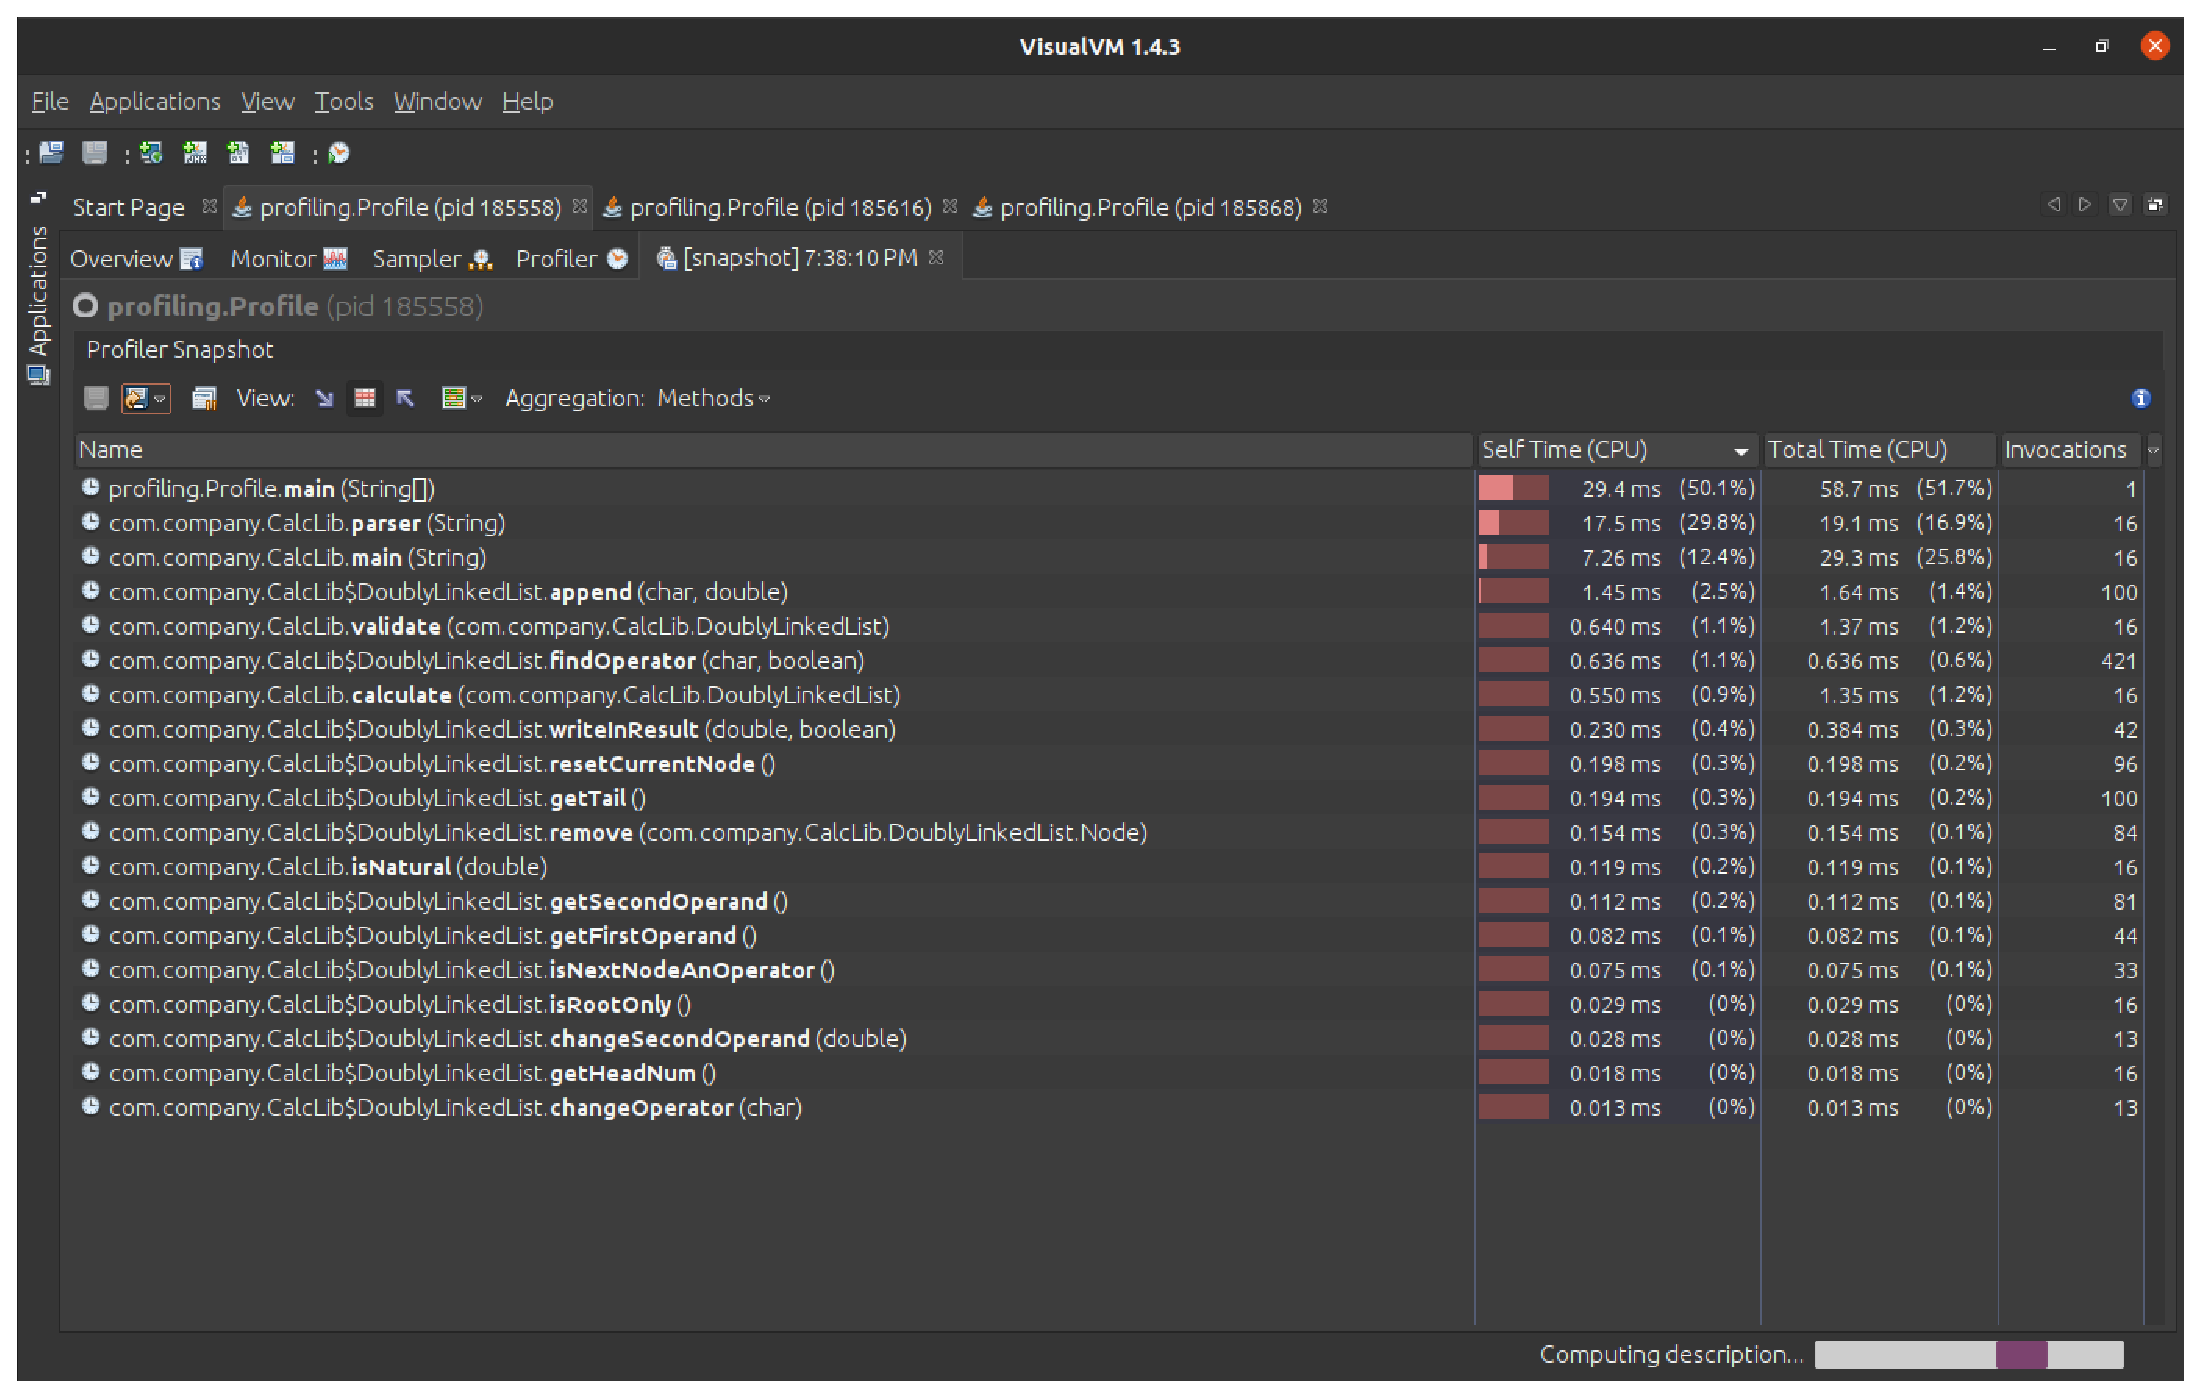
\includegraphics[width=16cm]{profiling_result-10_numbers.eps}
        \caption{Output of the profiler when calculating the standard deviation of \textbf{10} numbers}
      \end{center}
    \end{figure}

    In the picture we can clearly see that the library spent the most time 
    parsing the input (we should ignore the \texttt{profiling.Profile.main} method). 
    This is probably because of time-consuming operations with strings (mainly 
    when a root or a power is to be calculated). It still only took 17 milliseconds, 
    so I will conclude this after watching subsequent outputs. \\

    The \texttt{main} method also took some time (7 milliseconds), which is surprising,
    because it is \textit{fairly empty}. I suppose the only thing that could take a long
    time is figuring out in which format to print the result in. For example,
    instead of comparing the result to a constant, it is compared to $2^{52}$ 
    (accurate range of the double data type) which has to be computed. We will
    see if it changes in subsequent outputs.

    \newpage

    \begin{figure}[h]
      \begin{center}
        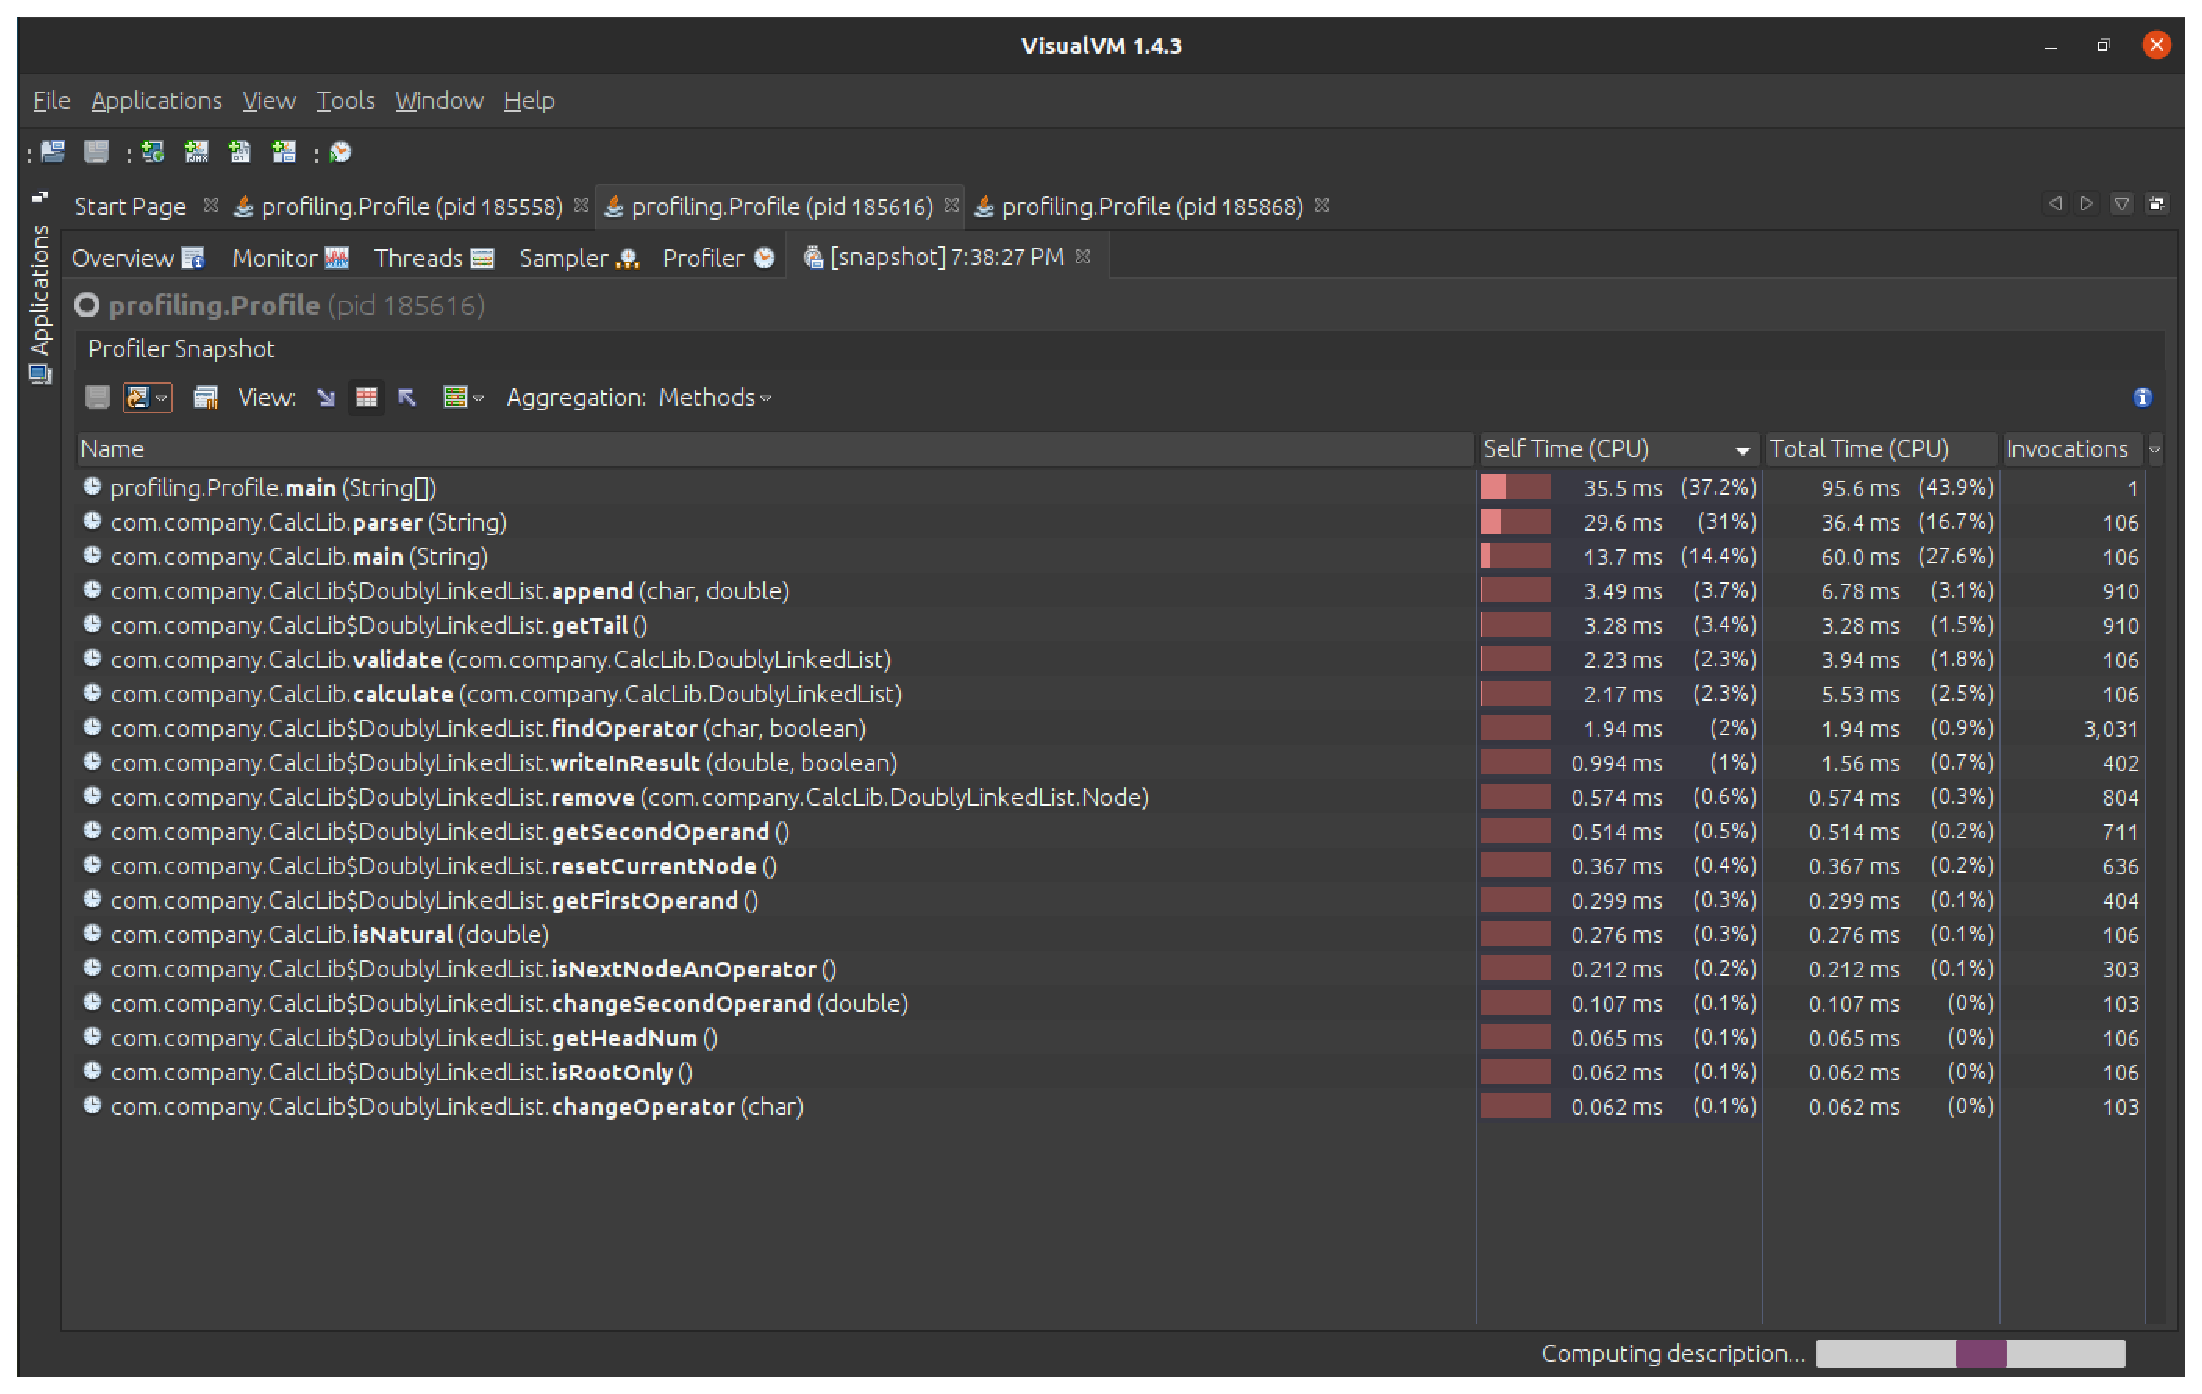
\includegraphics[width=16cm]{profiling_result-100_numbers.eps}
        \caption{Output of the profiler when calculating the standard deviation of \textbf{100} numbers}
      \end{center}
    \end{figure}

    We still see the \texttt{parser} method at the top (ignoring the 
    \texttt{profiling.Profile.main} method), which means that it is definitely worth
    optimising. Optimisation should be probably focused on more efficient ways 
    of working with strings, as there are actually too many calls (mainly) for 
    the \texttt{replace} method in the code. \\

    Six times more calls to the \texttt{main} method of \texttt{CalcLib} class were
    made compared to the previous figure (which was run with 10 times less 
    numbers), and the time doubled. This does not sound so bad, even when 
    scaled, but it is definitely worth looking into. I suppose
    it is taking too long exactly because of the computation of $2^{52}$, as
    I mentioned in the last paragraph. In this figure the \texttt{main} method from
    \texttt{CalcLib} class was called 106 times, which means that $2^{52}$ was calculated
    106 times\,\dots

    \newpage

    \begin{figure}
      \begin{center}
        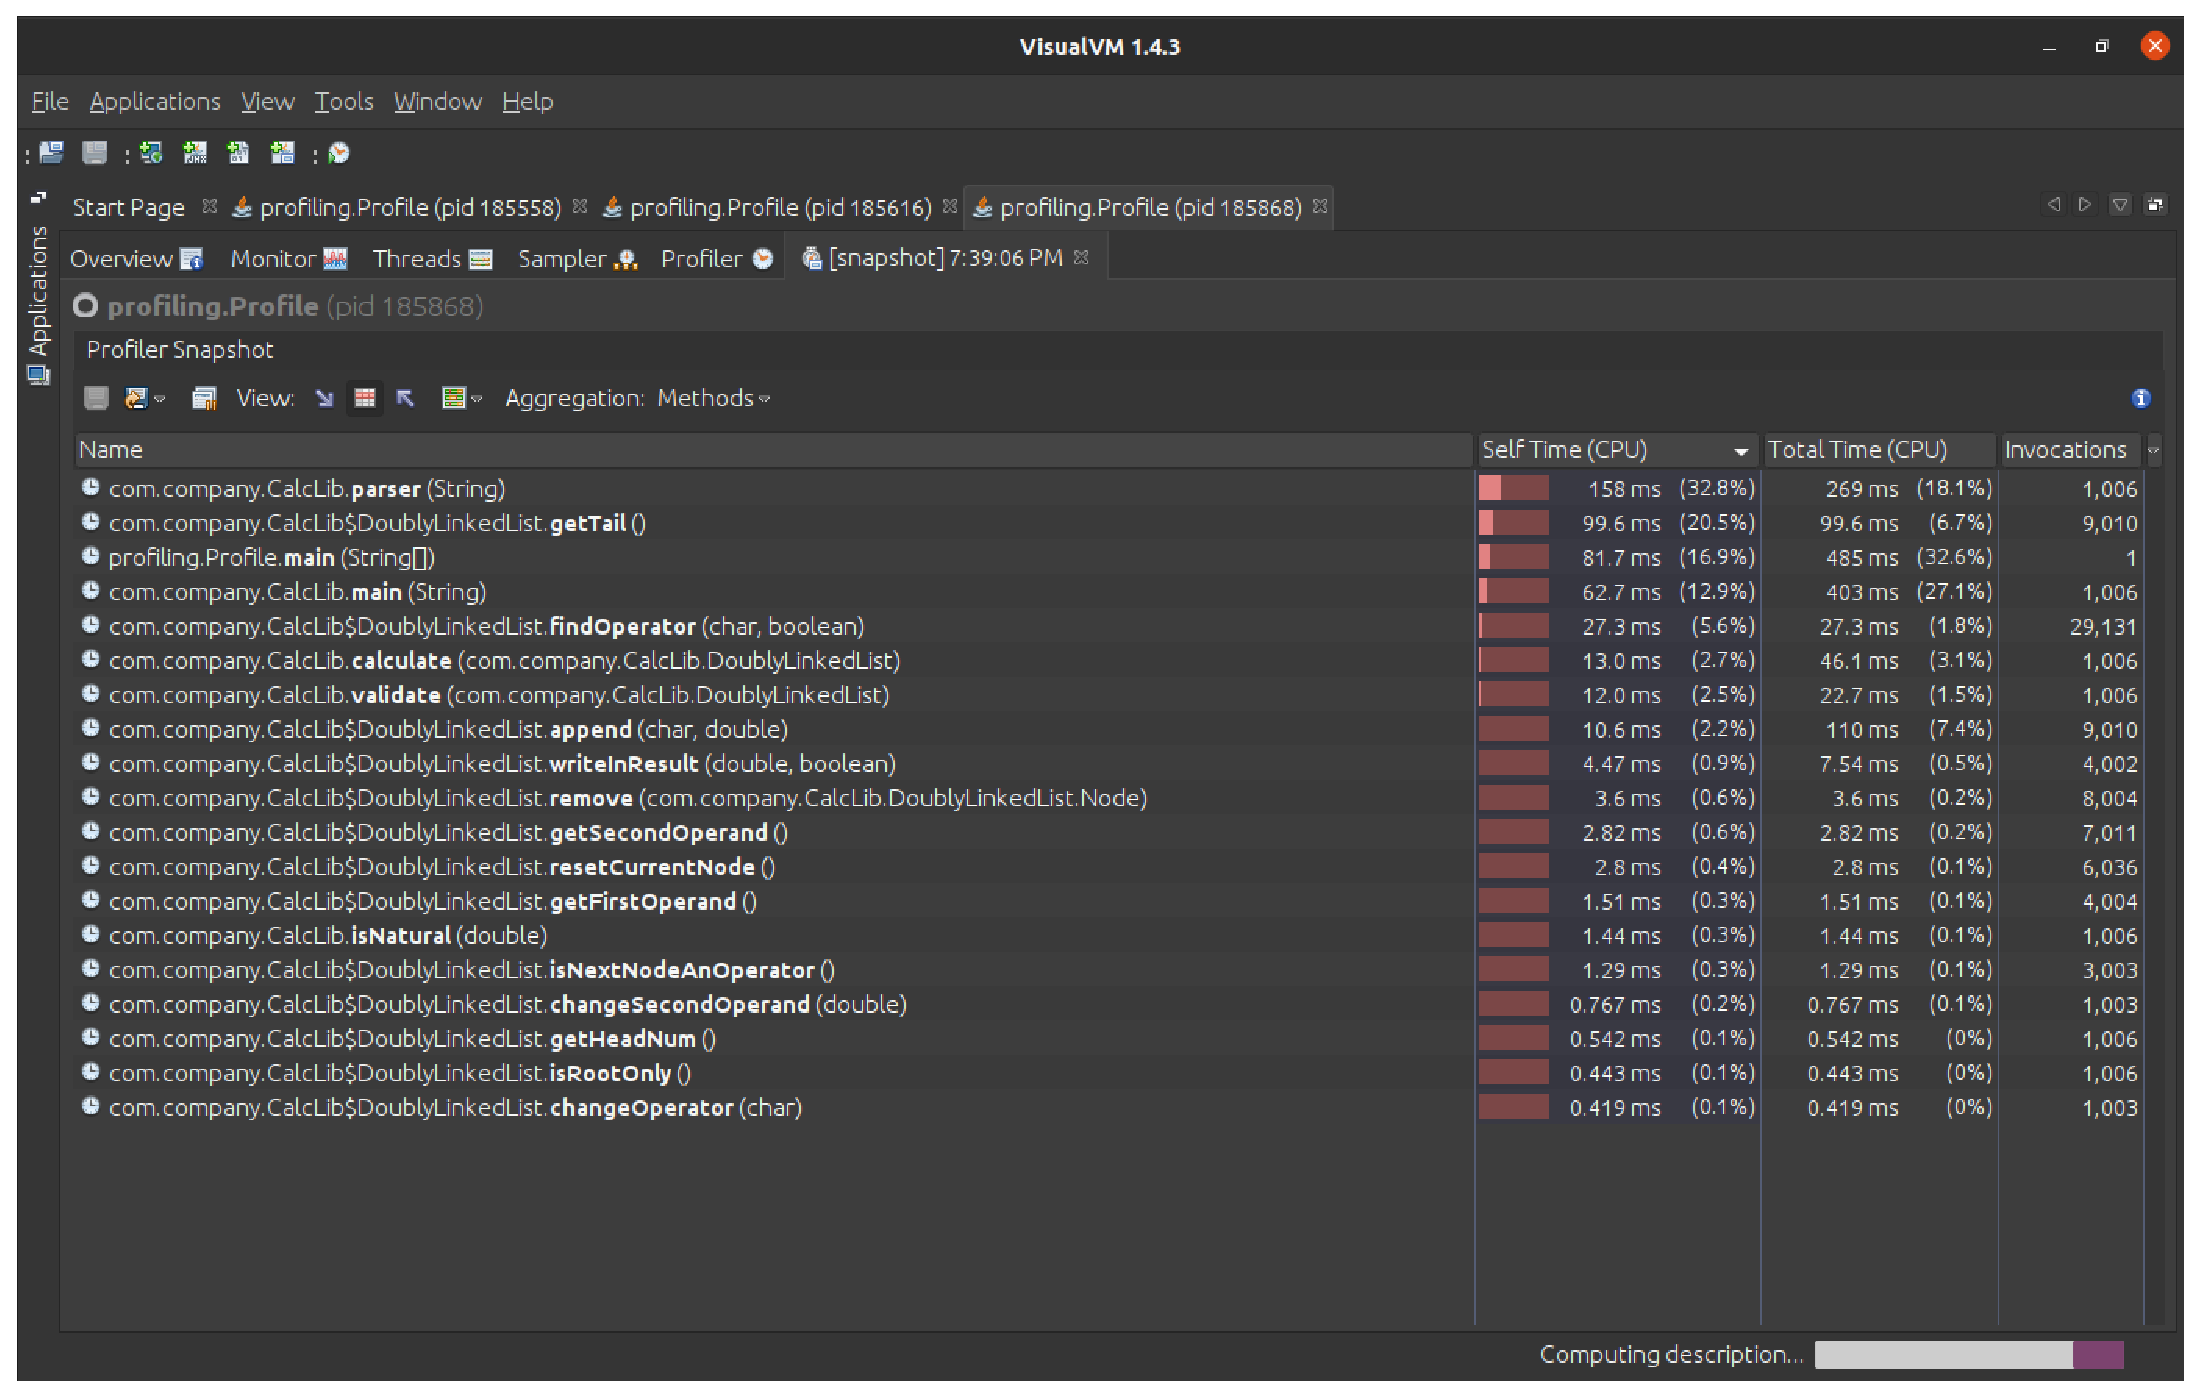
\includegraphics[width=16cm]{profiling_result-1000_numbers.eps}
        \caption{Output of the profiler when calculating the standard deviation of \textbf{1 000} numbers}
      \end{center}
    \end{figure}

    Calculating the standard deviation of 1000 numbers (mind that the 
    numbers are within range \textless 0, 1 000 000\textgreater) is 
    starting to take some time. \\

    The \texttt{parser} method still occupies the top of the list, which
    only proves my point it needs to be optimised. \\

    Surprisingly, though, \texttt{getTail} method jumped high and took
    100 milliseconds, which, to me, sounds like too long. I highly doubt
    a human would enter such a long expression for this to be a problem,
    but optimising this part should be really easy (although, the library
    could be used as a part of a different software, in which case, this
    definitely is a problem). The simplest and very efficient way to fix
    this would be to have a \texttt{Node tail} variable, which would be
    updated before every appending or removal of a node. That way, 
    \texttt{getTail} method would only return the \texttt{Node} pointer
    instead of searching through the whole list to find the end\,\dots

    \newpage

    \begin{figure}
      \begin{center}
        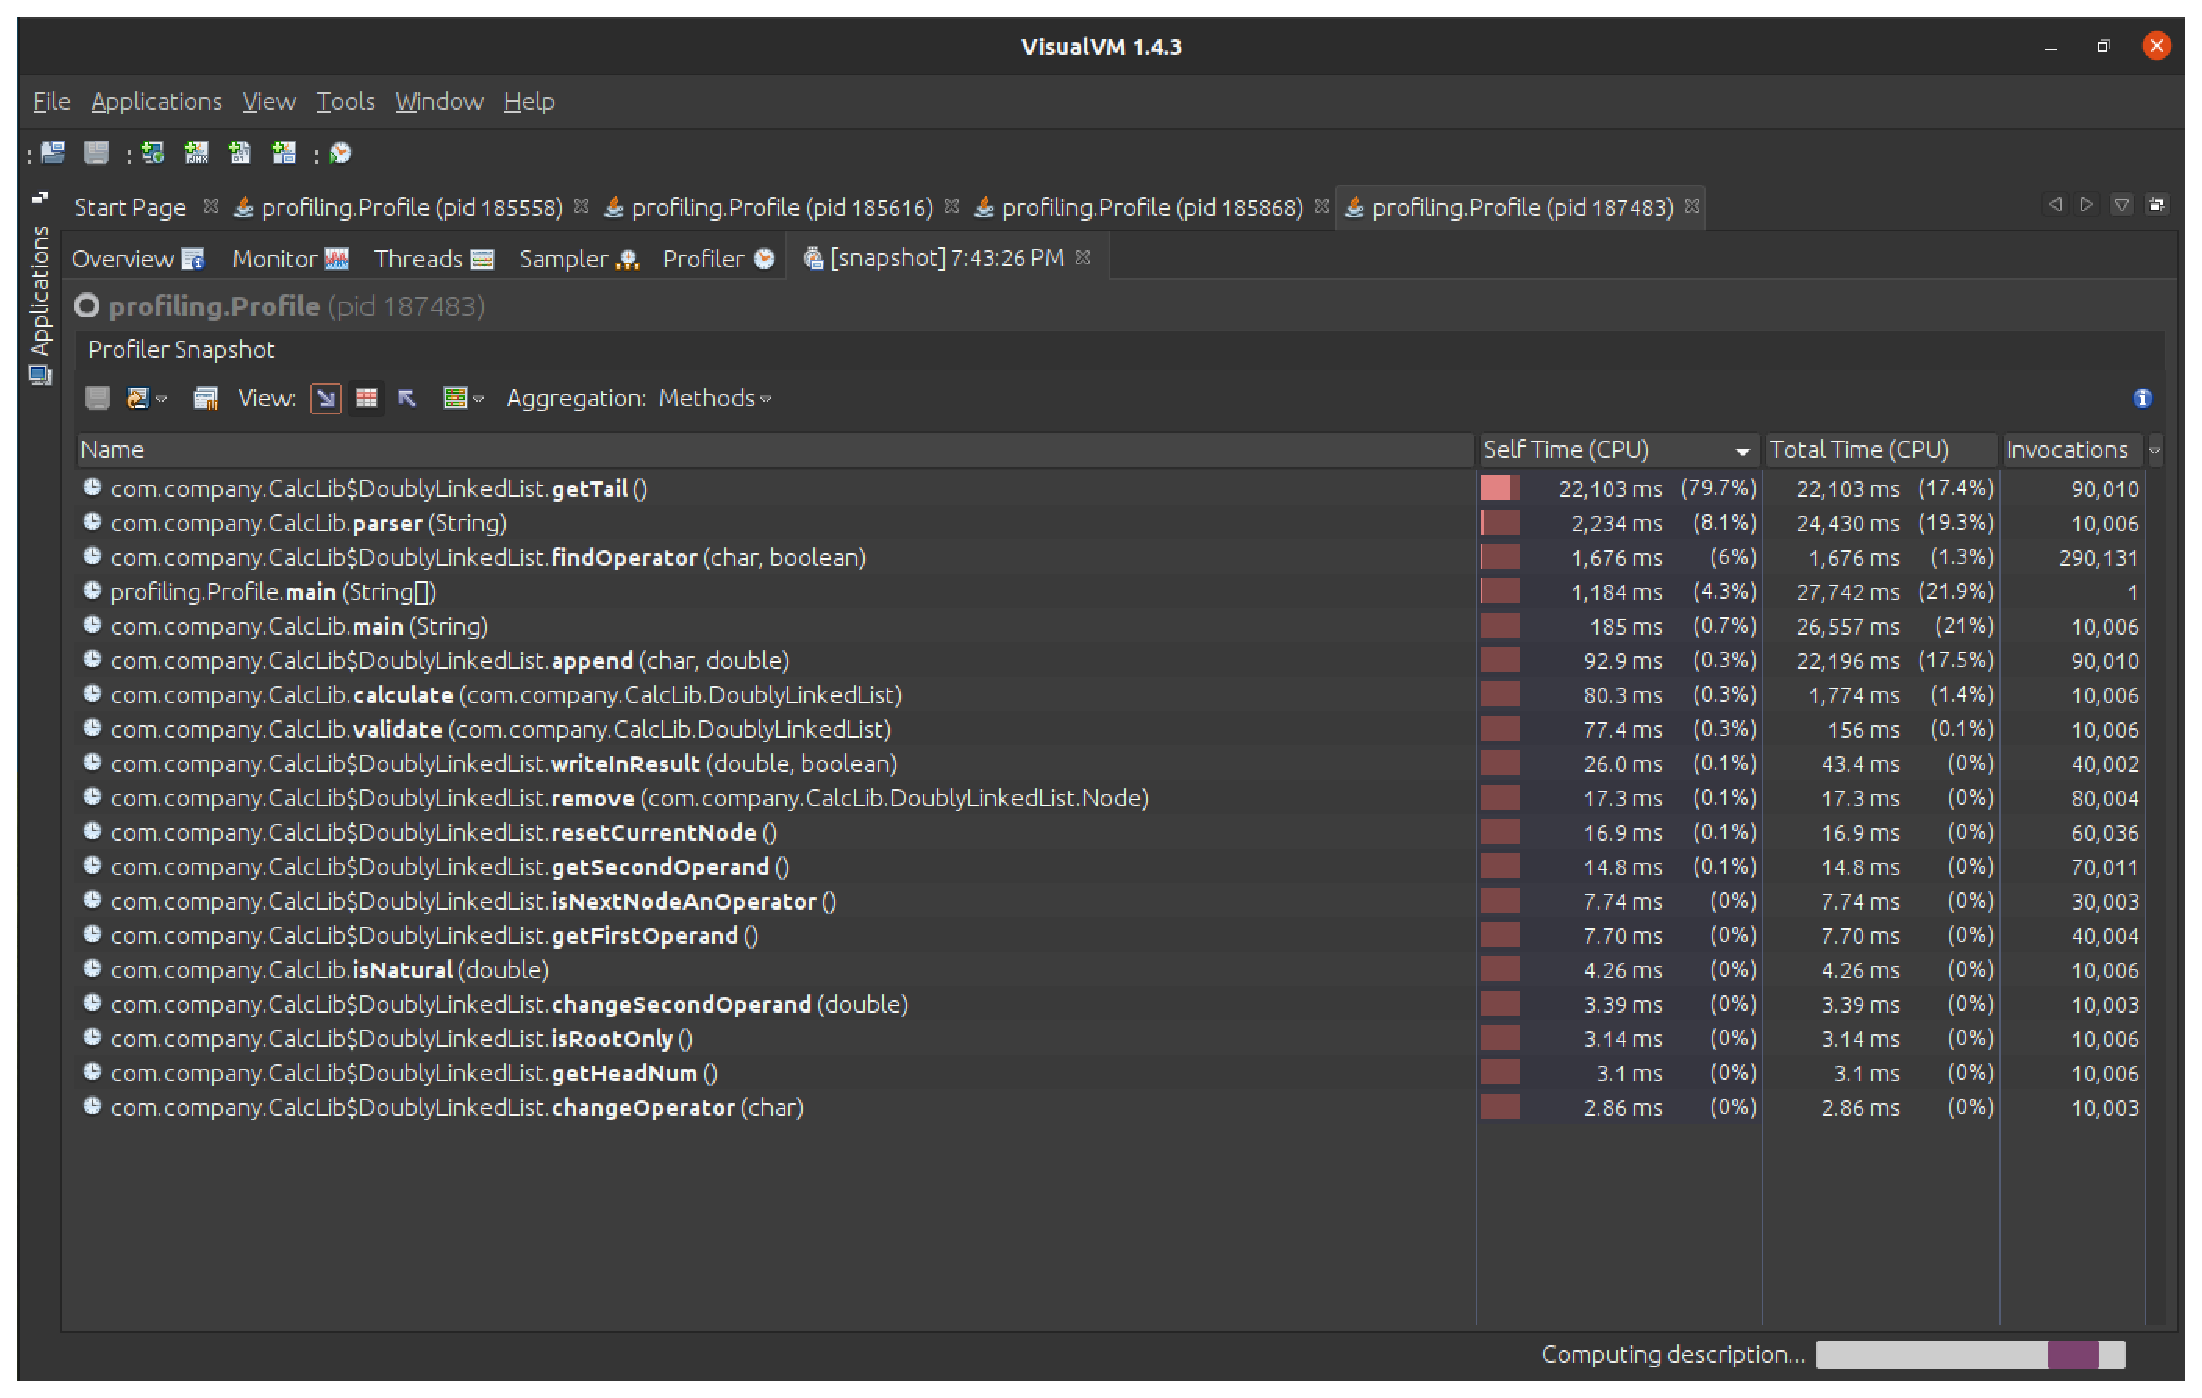
\includegraphics[width=16cm]{profiling_result-10000_numbers.eps}
        \caption{Output of the profiler when calculating the standard deviation of \textbf{10 000} numbers}
      \end{center}
    \end{figure}

    I understand that this is not a part of my job, but I wanted to include 
    the profiler output for 10 000 numbers as well. \\

    We can see that the \texttt{getTail} method is a huge problem since it took
    more than 22 seconds. \\

    The \texttt{parser} method still takes a lot of time, which proves it
    needs optimising. \\

    What is new here is the \texttt{findOperator} method, which took 1 676 
    milliseconds. It's not a big surprise, since it was called more than
    290 000 times. However, I don't see a simple way to optimise this method.
    Luckily, this doesn't seem like a big problem. We'd have to see
    the profiling output after optimisation of \texttt{getTail} and 
    \texttt{parser} to decide how severe this is. \\

    The \texttt{main} method in the library took \textit{only} 185 milliseconds
    this time, which, compared to the methods I mentioned above, is not
    much. I would try to optimise it anyways, but when thinking about
    scaling the library and while looking at these outputs, 185 milliseconds
    does not seem like a serious hold up.

    \newpage

    \begin{center}
    \large{Conclusion}
    \end{center}

    \bigskip

    \normalsize{Methods of the \texttt{CalcLib} class to optimise sorted by importance:}
    \begin{itemize}
      \item \texttt{getTail}
      \item \texttt{parser}
      \item \texttt{main}
      \item \texttt{findOperator}
    \end{itemize}

\end{document}
